\documentclass[titlepage,a4paper,12pt]{report}
\usepackage{amssymb,amsfonts,amsmath}
\usepackage{tikz}
\usetikzlibrary{arrows}
\newcommand\Interval[4]{%
  \begin{tikzpicture}[text height=1ex]%
    \draw[<-] (0,0) -- (1,0);
    \draw[{#3-#4}] (1,0) node[label=below:{#1}] {} -- (2,0) node[label=below:{#2}] {};
    \draw[->] (2,0) -- (3,0);
  \end{tikzpicture}
}
%\usepackage{fullpage}
\usepackage{graphicx}
%\usepackage[cc]{titlepic}
\usepackage{amsthm}
\newtheorem{definition}{Definition}[section]
\newtheorem{example}{Example}[section]
\newtheorem{theorem}{Theorem}[section]
\newtheorem{exercise}{Exercise}[section]
\newtheorem{corollary}{Corollary}[section]
\newtheorem{proposition}{Proposition}[section]
\pdfpagewidth 8.5in
\pdfpageheight 11in
\setlength\topmargin{-0.5in}
\setlength\headheight{0in}
\setlength\headsep{0in}
\setlength\textheight{9.5in}
\setlength\textwidth{7.0in}
\setlength\oddsidemargin{-0.5in}
\setlength\evensidemargin{1.0in}
\setlength\parindent{0.25in}
\setlength\parskip{0.25in}
%\begin{titlepage}
%\usepackage{titlepic}
%\titlepic{
\includegraphics[width=0.2\textwidth]{uz1.png}}
%
%\title{\textbf{HMTH111 Calculus 2}}
%\author{Nhawu. G\\
%		Department of Mathematics\\
%		University of Zimbabwe, ZIM}
%
%\end{titlepage}

\begin{document}
\begin{titlepage}
 
\begin{center}
 
 
% Upper part of the page

\includegraphics[width=0.15\textwidth]{uz1.png}\\[1cm]
 
\textsc{\LARGE University of Zimbabwe}\\[1.5cm]
 
\textsc{\Large HMTH101 CALCULUS 1}\\[0.5cm]
 
 
% Title

{ \huge \bfseries Calculus of Single Variables}\\[0.4cm]
 

 
% Author and supervisor
\begin{minipage}{0.4\textwidth}
\begin{center} \large
\emph{Author:}\\
G. \textsc{Nhawu}
\end{center}
\end{minipage}
\begin{minipage}{0.4\textwidth}
\begin{flushright} \large
\emph{Department:} \\
\textsc{Mathematics}
\end{flushright}
\end{minipage}

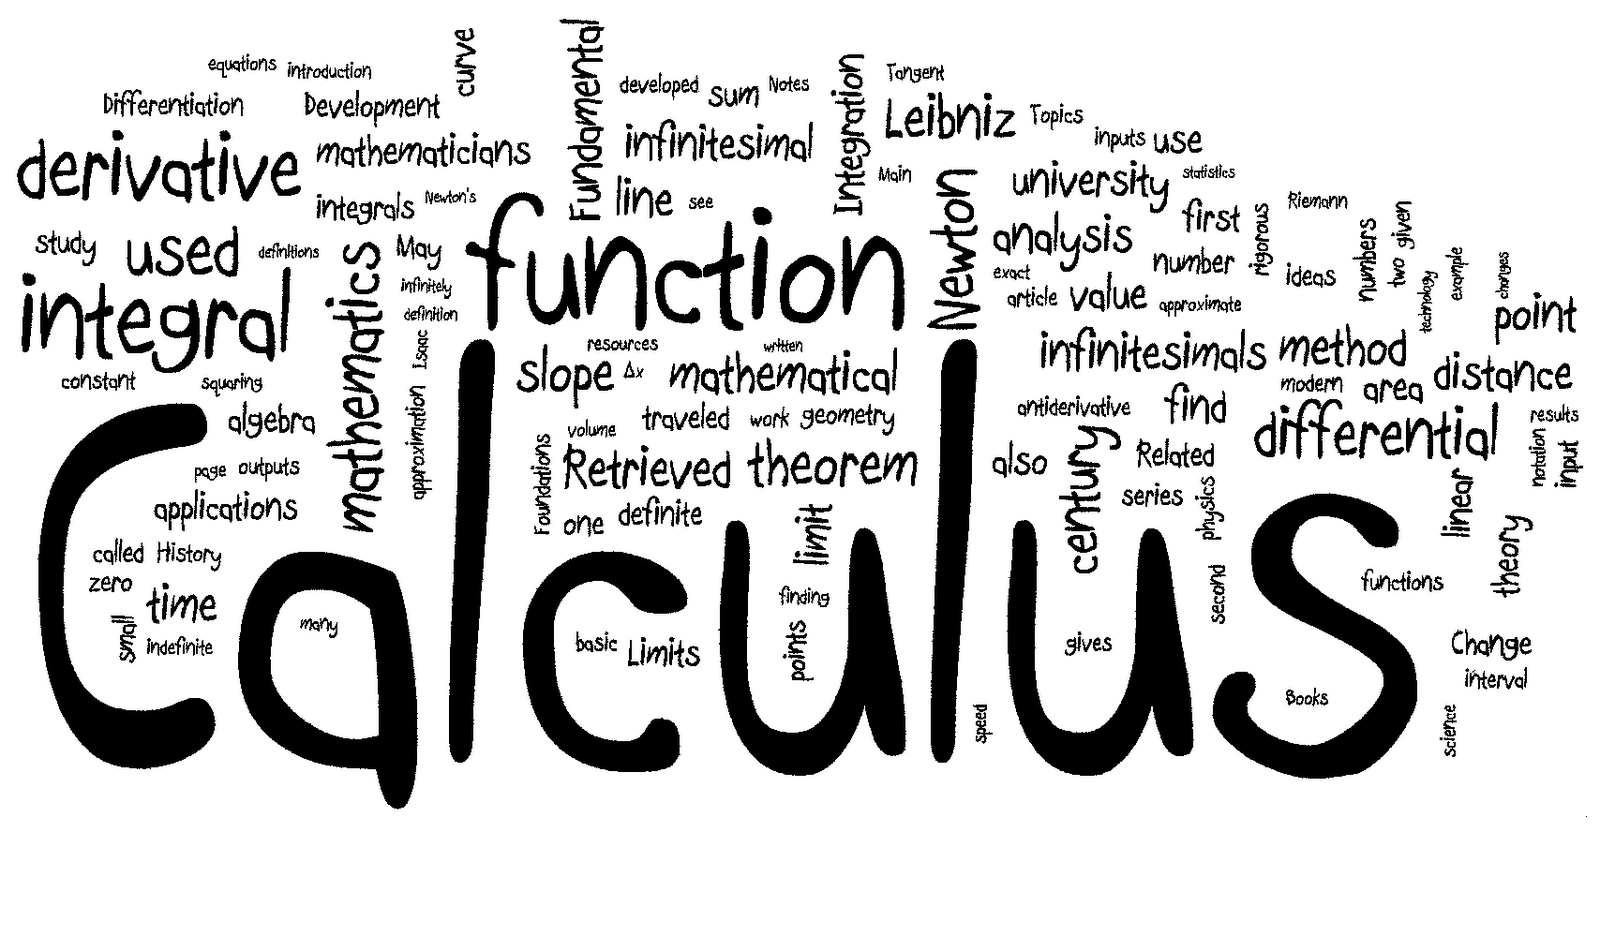
\includegraphics[width=0.98\textwidth]{calculus2.png}\\[1cm]
 \vfill
 
 
% Bottom of the page
{\large \today}
 
\end{center}
 
\end{titlepage}

\tableofcontents
\setcounter{chapter}{4}
\chapter{Differentiation}
\begin{center}
	\small{\parbox{18cm}{
		\begin{raggedright}
		{\small
		\textit{Any man who can drive safely while kissing a pretty girl is simply not giving the kiss the attention it deserves.}
 }
 
				\vspace{.5cm}\hfill{---Albert Einstein }
		\end{raggedright}
	}
} 
\end{center}
\textbf{Increments.} The \textit{increment} $\Delta x$ of a variable $x$ is the change in $x$ as it increases or decreases from one value $x=x_0$ to another value $x=x_1$ in its domain. Here, $\Delta x=x_1-x_0$ and we may write $x_1=x_0+\Delta x$. If the variable $x$ is given an increment $\Delta x$ from $x=x_0$ (i.e., if $x$ changes from $x=x_0$ to $x_1=x_0+\Delta x$) and a function $y=f(x)$ is thereby given an increment $\Delta y=f(x_0+\Delta x)-f(x_0)$ from $y=f(x_0)$, then the quotient 
\begin{equation*}
\dfrac{\Delta y} {\Delta x}=\dfrac{\hbox{change in}~~ y}{\hbox{change in }~ x}, 
\end{equation*}
is called the \textit{average rate of change} of the function on the interval between $x=x_0$ and $x_1=x_0+\Delta x$.
 
\noindent Let $f(x)$ be defined at any point $x_0$ in $(a,b)$. The derivative of $f(x)$ at $x=x_0$ is defined as 
\begin{equation*}
f'(x_0)=\lim _{h\rightarrow 0}\dfrac{f(x_0+h)-f(x_0)}{h}
\end{equation*}
if this limit exists. A function is called \textbf{differentiable} at a point $x=x_0$, if it has a derivative at that point, i.e., if $f'(x_0)$ exists.  If we write $x=x_0+h$, then $h=x-x_0$ and $h$ approaches $0$ if and only if $x$ approaches $x_0$. Therefore, an equivalent way of stating the definition of the derivative, is 
\begin{equation*}
f'(x_0)=\lim _{x\rightarrow x_0} \dfrac{f(x)-f(x_0)}{x-x_0}.
\end{equation*}

\noindent \textbf{Example:} If $f(x)=x^3-x$, find a formula for $f'(x)$.

\noindent \textbf{Solution:} 
\begin{eqnarray*}
f'(x) &=& \lim _{h\rightarrow 0} \dfrac{f(x+h)-f(x)}{h} =\lim _{h\rightarrow 0}\dfrac{[(x+h)^3-(x+h)]-[x^3-x]}{h}\\
&=& \lim _{h\rightarrow 0} \dfrac{x^3+3x^2h+3xh^2+h^3-x-h-x^3+x}{h}\\
&=& \lim _{h\rightarrow 0} \dfrac{3x^2h+3xh^2+h^3-h}{h}\\
&=& \lim _{h\rightarrow 0} (3x^2+3xh+h^2-1) =3x^2-1.
\end{eqnarray*}

\noindent \textbf{Example:} If $f(x)=\sqrt{x}$, find the derivative of $f$.

\noindent \textbf{Solution:} 
\begin{eqnarray*}
f'(x) &=& \lim _{h\rightarrow 0} \dfrac{f(x+h)-f(x)}{h}\\
&=& \lim _{h\rightarrow 0} \dfrac{\sqrt{x+h}-\sqrt{x}}{h}\\
&=& \lim _{h\rightarrow 0} \dfrac{\sqrt{x+h}-\sqrt{x}}{h} \cdot \dfrac{\sqrt{x+h}+\sqrt{x}}{\sqrt{x+h}-\sqrt{x}}\\
&=& \lim _{h\rightarrow 0} \dfrac{(x+h)-x}{h(\sqrt{x+h}+\sqrt{x})}\\
&=& \lim _{h\rightarrow 0} \dfrac{1}{\sqrt{x+h}+\sqrt{x}}\\
&=& \dfrac{1}{\sqrt{x} +\sqrt{x}} =\dfrac{1}{2\sqrt{x}}. 
\end{eqnarray*}
\noindent The derivative at $x$ may be denoted by $f'(x)$, $y'$, $\dfrac{dy}{dx}$, $\dfrac{d}{dx}(f(x))$. The symbol $\dfrac{d}{dx}$ is called \textbf{differentiation operator} because it indicates the operation of \textbf{differentiation}. The process of finding derivatives of functions is called \textbf{differentiation}.

\noindent  A function $f$ is differentiable at $x_0$ if $f'(x_0)$ exists. It is \textbf{differentiable on an open interval} $(a,b)$ [or $(a,\infty)$ or $(-\infty , a)$ or $(-\infty , \infty)$], if it is differentiable at every number in the interval.

\noindent \textbf{Example:} Where is the function $f(x)=|x|$ differentiable?

\noindent \textbf{Solution:} If $x>0$, then $|x|=x$ and we can choose $h$ small enough that $x+h>0$ and hence $|x+h|=x+h$. Therefore, for $x>0$, 
\begin{eqnarray*}
f'(x) &=& \lim _{h\rightarrow 0}\dfrac{|x+h|-|x|}{x}\\
&=&\lim _{h\rightarrow 0} \dfrac{(x+h)-x}{h}=\lim _{h\rightarrow 0}\dfrac{h}{h}=1,
\end{eqnarray*}
and so $f$ is differentiable for any $x>0$. 

\noindent Similarly, for $x<0$, we have $|x|=-x$ and $h$ can be chosen small enough that $x+h<0$ and so $|x+h|=-(x+h)$. Therefore, for $x<0$, 
\begin{eqnarray*}
f'(x) &=& \lim _{h\rightarrow 0}\dfrac{|x+h|-|x|}{h}\\
&=& \lim _{h\rightarrow 0}\dfrac{-(x+h)-(-x)}{h} =\lim _{h\rightarrow 0} \dfrac{-h}{h}=-1,
\end{eqnarray*} 
and so $f$ is differentiable for any $x<0$. 

\noindent For $x=0$ we have to investigate 
\begin{eqnarray*}
f'(0) &=& \lim _{h\rightarrow 0}\dfrac{f(0+h)-f(0)}{h}\\
&=& \lim _{h\rightarrow 0} \dfrac{|0+h|-|0|}{h} \quad (\hbox{if it exists}). 
\end{eqnarray*}
Let's compute the left and right limits separately;
\begin{eqnarray*}
\lim _{h\rightarrow 0^+} \dfrac{|0+h|-|0|}{h} &=& \lim _{h\rightarrow 0^+}\dfrac{|h|}{h}=\lim _{h\rightarrow 0^+} 1=1.\\
\lim _{h\rightarrow 0^-} \dfrac{|0+h|-|0|}{h} &=& \lim _{h\rightarrow 0^-}\dfrac{|h|}{h}=\lim _{h\rightarrow 0^-} (-1)=-1.
\end{eqnarray*}
Since these limits are different $f'(0)$ does not exist.  Thus, $f$ is differentiable at all $x$ except $0$.
\section{Differentiation Techniques (Finding Derivatives)}
\begin{enumerate}
\item \begin{equation*}
f'(x_0)=\lim _{h\rightarrow 0}\dfrac{f(x_0+h)-f(x_0)}{h}
\end{equation*}
if this limit exists.
\item The derivative of any constant function is zero, i.e., $c'=0$.
\item For any real number $n$, 
\begin{equation*}
(x^n)'=nx^{n-1}.
\end{equation*}
When differentiating, results can be expressed in a number of ways. For example, (i)\, if $y=3x^2$ then $\dfrac{dy}{dx}=6x$, \quad (ii)\, if $f(x)=3x^2$ then $f'(x)=6x$, \quad (iii)\, the differential coefficient of $3x^2$ is $6x$. \\
For example, if $f(x)=\sqrt{x}=x^{\frac{1}{2}}$, then $f'(x)=\dfrac{1}{2}x^{\frac{1}{2}-1}=\frac{1}{2}x^{-\frac{1}{2}}=\dfrac{1}{2\sqrt{x}}$.\\
\textbf{You Try It:} Using the general rule, differentiate the following with respect to $x$ :\\ (a)\, $f(x)=5x^7$ \quad (b)\, $f(x)=\dfrac{4}{x^2}$.
\item For any constant $c$, $(cf(x))'=cf'(x)$. For example, $(5x^3)'=5(x^3)'=5(3x^2)=15x^2$.
\item The derivative of a sum (difference) is the sum (difference) of the derivatives, 
\begin{equation*}
(f(x)\pm g(x))'=f'(x)\pm g'(x).
\end{equation*}
For example, \[(3x^5-2x^2+1)'=(3x^5)'-(2x^2)'+1'=3(x^5)'-2(x^2)'+0=3(5x^4)-2(2x)=15x^4-4x.\]
\item Product Rule 
\begin{equation*}
(f(x)g(x))'=f(x)g'(x)+g(x)f'(x).
\end{equation*}
\item Quotient Rule
\begin{equation*}
\left(\dfrac{f(x)}{g(x)}\right)'=\dfrac{g(x)f'(x)-f(x)g'(x)}{(g(x))^2}.
\end{equation*}
\item \textbf{Parametric Equations.} If the coordinates $(x,y)$ of a point $P$ on a curve are given as functions $x=f(u)$ and $y=g(u)$ of a third variable or \textit{parameter} $u$, the equations $x=f(u)$ and $y=g(u)$ are called \textit{parametric equations of the curve}. For example, $x=\frac{1}{2}t, \, y=4-t^2$ or $x=\cos \theta, \, y=4\sin ^2 \theta$.

\noindent \textbf{The First Derivative} $\dfrac{dy}{dx}$ is given by 
\begin{equation*}
\dfrac{dy}{dx} =\dfrac{dy/ du}{dx/ du}.
\end{equation*}
\textbf{The Second Derivative} $\dfrac{d^2y }{dx^2}$ is given by 
\begin{equation*}
\dfrac{d^2y}{dx^2} =\dfrac{d}{du}\left( \dfrac{dy}{dx}\right)\dfrac{du}{dx}.
\end{equation*}
\textbf{Example:} Find $\dfrac{dy}{dx}$ and $\dfrac{d^2y}{dx^2}$ given $x=\theta-\sin \theta$ and $y=1-\cos \theta$.

\noindent \textbf{Solution:} Note that $\dfrac{dx}{d\theta}=1-\cos \theta$ and $\dfrac{dy}{d\theta}=\sin \theta$, so 
\begin{equation*}
\dfrac{dy}{dx} =\dfrac{dy/ d\theta}{dx/ d\theta}=\dfrac{\sin \theta}{1-\cos \theta}.
\end{equation*}
Also \begin{eqnarray*}
\dfrac{d^2y}{dx^2} &=& \dfrac{d}{d\theta}\left( \dfrac{\sin \theta}{1-\cos \theta}\right)\dfrac{d\theta}{dx}\\
&=& \dfrac{\cos \theta -1}{(1-\cos \theta)^2}\cdot \dfrac{1}{1-\cos \theta} =-\dfrac{1}{(1-\cos \theta)^2}.
\end{eqnarray*}
\textbf{Example:} Find $\dfrac{dy}{dx}$ and $\dfrac{d^2y}{dx^2}$ given $x=e^t\cos t$ and $y=e^t\sin t$.

\noindent \textbf{Solution:} Note that $\dfrac{dx}{dt}=e^t(\cos t -\sin t)$ and $\dfrac{dy}{dt}=e^t(\sin t +\cos t)$, so 
\begin{equation*}
\dfrac{dy}{dx} =\dfrac{dy/ dt}{dx/ dt}=\dfrac{\sin t +\cos t}{\cos t -\sin t}.
\end{equation*}
Also 
\begin{eqnarray*}
\dfrac{d^2y}{dx^2} &=& \dfrac{d}{dt}\left(\dfrac{\sin t +\cos t}{\cos t -\sin t} \right)\dfrac{dt}{dx}\\
&=& \dfrac{2}{(\cos t - \sin t)^2} \cdot \dfrac{1}{e^t(\cos t -\sin t)} =\dfrac{2}{e^t(\cos t -\sin t)^3}.
\end{eqnarray*}
\end{enumerate}
\begin{theorem}
If $f(x)=c$ is a constant function, then $f'(x)=0$ for all real numbers $x$. 
\end{theorem}
\begin{proof}
Observe that $f'(x)=\displaystyle \lim _{h\rightarrow 0}\dfrac{f(x+h)-f(x)}{h}=\displaystyle \dfrac{c-c}{h}=0$.
\end{proof}
\begin{theorem}[Product Rule]
If $f$ and $g$ are both differentiable at $x$, then the product function $fg$ is also differentiable at $x$ and $(fg)'(x)=f(x)g'(x)+g(x)f'(x)$.
\end{theorem}
\begin{proof}
\begin{equation*}
(fg)'(x)=\lim _{h\rightarrow 0}\dfrac{f(x+h)g(x+h)-f(x)g(x)}{h}.
\end{equation*}
Trick of adding and subtracting $f(x+h)g(x)$ to the numerator,
\begin{eqnarray*}
\lim _{h\rightarrow 0}\dfrac{f(x+h)g(x+h)-f(x+h)g(x)+f(x+h)g(x)-f(x)g(x)}{h} &=&\\
\lim _{h\rightarrow 0} {f(x+h)}\lim _{h\rightarrow 0}\dfrac{g(x+h)-g(x)}{h}+g(x)\lim _{h\rightarrow 0}\dfrac{f(x+h)-f(x)}{h} &=&\\
f(x)g'(x)+g(x)f'(x).
\end{eqnarray*}
\end{proof}
\begin{theorem}
If $g$ is differentiable at $x$ and $g(x)\neq 0$, then 
\begin{equation*}
\left(\dfrac{1}{g}\right)'(x)=-\dfrac{g'(x)}{(g(x))^2}.
\end{equation*}
\end{theorem}
\begin{proof}
\begin{eqnarray*}
\lim _{h\rightarrow 0} \dfrac{\frac{1}{g(x+h)}-\frac{1}{g(x)}}{h} &=& \lim _{h\rightarrow 0}\dfrac{g(x)-g(x+h)}{h(g(x))(g(x+h))}\\
&=& \lim _{h\rightarrow 0} \dfrac{-(g(x+h)-g(x))}{h}\dfrac{1}{g(x)g(x+h)}\\
&=& \lim _{h\rightarrow 0} \dfrac{-(g(x+h)-g(x))}{h} \lim _{h\rightarrow 0}\dfrac{1}{g(x)g(x+h)}\\
&=& -g'(x)\dfrac{1}{(g(x))^2}.
\end{eqnarray*}
\end{proof}
\begin{theorem}
If $f$ and $g$ are differentiable at $x$ and $g(x)\neq 0$, then $\dfrac{f}{g}$ is differentiable at $x$ and 
$\left(\dfrac{f}{g}\right)'(x)=\dfrac{g(x)f'(x)-f(x)g'(x)}{(g(x))^2} $.
\end{theorem}
\begin{proof}
Since $\dfrac{f}{g}=f\left(\dfrac{1}{g}\right)$, we have
\begin{eqnarray*}
\left(\dfrac{f}{g}\right)'(x) &=&\left(f\cdot \dfrac{1}{g}\right)'(x)\\
&=& f'(x)\dfrac{1}{g(x)}+f(x)\left(\dfrac{1}{g}\right)'(x)\\
&=& \dfrac{f'(x)}{g(x)}+f(x)\left(-\dfrac{g'(x)}{(g(x))^2}\right)\\
&=& \dfrac{f'(x)g(x)-f(x)g'(x)}{(g(x))^2}.
\end{eqnarray*}
\end{proof}
\textbf{Example:} $f(x)=\dfrac{x^2-1}{x^2+1}$, then $f'(x)=\dfrac{(x^2+1)(2x)-(x^2-1)(2x)}{(x^2+1)^2}=\dfrac{4x}{(x^2+1)^2}$.

\noindent \textbf{Example:} If $f(x)=\dfrac{x}{x^2+1}$, then $f'(x)=\dfrac{(x^2+1)-x(2x)}{(x^2+1)^2}=\dfrac{1-x^2}{(x^2+1)^2}$.

\noindent \textbf{Example:} If $f(x)=\dfrac{1}{x}$, then $f'(x)=-\dfrac{1}{x^2}$.

\noindent \textbf{Example:} If $x=\cos t$ and $y=t\sin t$, find $\dfrac{dy}{dx}$.

\noindent \textbf{Solution:} \begin{equation*}
\dfrac{dy}{dx}=\dfrac{\dfrac{d}{dt}(t\sin t)}{\dfrac{d}{dt}(\cos t)}=\dfrac{\sin t+t\cos t}{-\sin t}.
\end{equation*}
\section{Derivatives of Trigonometric Functions}
Recall : 
\begin{equation*}
\lim _{h\rightarrow 0} \dfrac{\sin h}{ h}=1 \quad \hbox{and} \quad \lim _{h\rightarrow 0} \dfrac{1-\cos h}{h}=0.
\end{equation*}
\begin{eqnarray*}
(\sin x)' &=& \lim _{h\rightarrow 0} \dfrac{\sin (x+h)-\sin x}{h}\\
&=& \lim _{h\rightarrow 0} \dfrac{\sin x \cos h +\cos x \sin h -\sin x}{h}\\
&=& \lim _{h\rightarrow 0} \dfrac{\sin x (\cos h-1)+\cos x \sin h}{h}\\
&=& \lim _{h\rightarrow 0} \left(-\sin x \dfrac{(1-\cos h)}{h}+\left(\cos x\dfrac{\sin h}{h}\right)\right)\\
&=& -\sin x (0)+\cos x (1).
\end{eqnarray*}
Hence $(\sin x)'=\cos x$.

\noindent \textbf{Example:} Find $\dfrac{dy}{dx}$ if $y=x^3\sin x$.

\noindent \textbf{Solution:} $\dfrac{dy}{dx}=(x^3\sin x)'=x^3(\sin x)'+\sin x (x^3)'=x^3\cos x +3x^2\sin x$.

\noindent \textbf{Example:} Determine whether the function, 
\[ f(x) = \left\{ 
\begin{array}{l l}
  x^3\sin \left(\dfrac{1}{x}\right), & \quad \hbox{if}~~~ x\neq 0 \\
 0, & \quad \hbox{if}~~~ x=0,\\ \end{array} \right. \]
 is differentiable at $x=0$.
 
\noindent \textbf{Solution:}  Observe that 
\begin{equation*}
\lim _{h\rightarrow 0} \dfrac{h^3\sin \frac{1}{h}-0}{h}=\lim _{h\rightarrow 0}h^2\sin \frac{1}{h}=0.
\end{equation*}

\noindent \textbf{Logarithmic Functions.} Assume $a>0$ and $a\neq 1$. If $a^y=x$, then define $y=\log _a x$. Let $\ln x \equiv \log _e x$ ($\ln x$ is called the \textit{natural logarithm} of $x$).

\noindent \textbf{Basic Properties of Logarithms}
\begin{enumerate}
\item $\log _a 1 =0$ (In particular, $\ln 1 =0$).
\item $\log _a a=1$ (In particular, $\ln e =1$).
\item $\log _a uv=\log _a u +\log _a v$.
\item $\log _a \left(\dfrac{u}{v}\right)=\log _a u-\log _a v$.
\item $\log _a u^r =r\log _a u$.
\end{enumerate}

\noindent \textbf{Derivatives of $\ln x$ and $e^x$} are $\dfrac{d}{dx}e^x=e^x$ and $\dfrac{d}{dx}\ln x =\dfrac{1}{x}$. Also $\dfrac{d}{dx}(a^x)=a^x\ln x, \, a>0$.

\noindent \textbf{Example:} Calculate the derivative $\dfrac{d}{dx}[(\sin x +x)\cdot (x^3-\ln x)]$.

\noindent \textbf{Solution:}  We know that $\dfrac{d}{dx} \sin x =\cos x, \dfrac{d}{dx} x=1, \, \dfrac{d}{dx}x^3=3x^2$ and $\dfrac{d}{dx}\ln x =\dfrac{1}{x}$. Therefore, by the addition rule, 
\begin{equation*}
\dfrac{d}{dx} (\sin x +x) =\dfrac{d}{dx}\sin x +\dfrac{d}{dx} x =\cos x +1
\end{equation*} 
and 
\begin{equation*}
\dfrac{d}{dx} (x^3-\ln x)=\dfrac{d}{dx}x^3-\dfrac{d}{dx}\ln x =3x^2-\dfrac{1}{x}.
\end{equation*}
Now we may conclude the calculation by applying the product rule;
\begin{eqnarray*}
\dfrac{d}{dx}[(\sin x +x)\cdot(x^3-\ln x)] &=& \dfrac{d}{dx} (\sin x +x)\cdot (x^3-\ln x) +(\sin x +x)\cdot \dfrac{d}{dx}(x^3-\ln x)\\
&=& (\cos x +1)\cdot (x^3-\ln x) +(\sin x +x)\cdot \left(3x^2-\dfrac{1}{x}\right)\\
&=& 4x^3-1 +x^3\cos x +3x^2\sin x -\dfrac{1}{x}\sin x -\ln x \cos x -\ln x. 
\end{eqnarray*}

\noindent \textbf{You Try It:} Calculate the derivative 
\begin{equation*}
\dfrac{d}{dx}\left(\sin x \cdot \left( \cos x -\dfrac{x}{e^x+\ln x}\right)\right).
\end{equation*}
\section{Derivative of a Composition [The Chain Rule]}
We calculate the derivative of a composition by 
\begin{equation*}
[f\circ g(x)]'=f'(g(x))\cdot g'(x).
\end{equation*}
If $y=f(u)$ where $u=g(x)$, then 
\begin{equation*}
\dfrac{dy}{dx}=\dfrac{dy}{du}\cdot \dfrac{du}{dx}=f'(u)\dfrac{du}{dx}=f'(g(x))g'(x).
\end{equation*}
Similarly, if $y=f(u)$ where $u=g(v)$ and $v=h(x)$, then 
\begin{equation*}
\dfrac{dy}{dx}=\dfrac{dy}{du}\cdot \dfrac{du}{dv}\cdot \dfrac{dv}{dx}.
\end{equation*}

\noindent \textbf{Example:} Calculate the derivative $\dfrac{d}{dx}(\sin (x^3-x^2))$.

\noindent \textbf{Solution:}  This is the composition of functions, so we must apply the Chain Rule.  It is essential to recognize what function will play the role of $f$ and what function will play the role of $g$. Notice that, if $x$  is the variable, then $x^3-x^2$ is applied first and $\sin$ applied next. So it must be that $g(x)=x^3-x^2$ and $f(s)=\sin s$. Notice that $\dfrac{d}{ds}f(s)=\cos s$ and $\dfrac{d}{dx}g(x)=3x^2-2x$. Then 
\begin{equation*}
\sin (x^3-x^2) =f\circ g(x)
\end{equation*}
and \begin{eqnarray*}
\dfrac{d}{dx}(\sin (x^3-x^2)) &=& \dfrac{d}{dx}(f\circ g(x))\\
&=& \left[\dfrac{df}{ds}(g(x)) \right]\cdot \dfrac{d}{dx}g(x)\\
&=& \cos (g(x)) \cdot (3x^2-2x)\\
&=& [\cos (x^3-x^2)]\cdot (3x^2-2x).
\end{eqnarray*}

\noindent \textbf{Example:} Calculate the derivative $\dfrac{d}{dx}\ln \left(\dfrac{x^2}{x-2}\right)$.

\noindent \textbf{Solution:} Let $h(x)=\ln \left(\dfrac{x^2}{x-2}\right)$. Then $h=f\circ g$, where $f(s)=\ln s$ and $g(x)=\dfrac{x^2}{x-2}$.  So $\dfrac{d}{ds}f(s)=\dfrac{1}{s}$ and $\dfrac{d}{dx} g(x)=\dfrac{(x-2)\cdot 2x-x^2\cdot 1}{(x-2)^2}=\dfrac{x^2-4x}{(x-2)^2}$. As a result, 
\begin{eqnarray*}
\dfrac{d}{dx}h(x) &=& \dfrac{d}{dx} (f\circ g)\\
&=& \left[\dfrac{df}{ds}(g(x)) \right]\cdot \dfrac{d}{dx}g(x)\\
&=& \dfrac{1}{g(x)}\cdot \dfrac{x^2-4x}{(x-2)^2}\\
&=& \dfrac{1}{\dfrac{x^2}{x-2}} \cdot \dfrac{x^2-4x}{(x-2)^2}\\
&=& \dfrac{x-4}{x(x-2)}.
\end{eqnarray*}

\noindent \textbf{You Try It:} Calculate the derivative of $\tan (e^x-x)$.
\section{Continuity and Differentiation}
What is the relationship between continuity and differentiation? It appears that functions that have derivatives must be continuous.
\begin{theorem}
If a function  $f$ is differentiable at a point $x$, then it is continuous at $x$.
\end{theorem}
\begin{proof}
We want to show that $f$ is continuous at $x$, i.e., $\displaystyle \lim _{t\rightarrow x} f(t)=f(x)$ or $\displaystyle \lim _{h\rightarrow 0} f(x+h)=f(x)$, where $h=t-x$. It will be sufficient to show that $\displaystyle \lim _{h\rightarrow 0} [f(x+h)-f(x)]=0$.

\noindent Now, 
\begin{eqnarray*}
\lim _{h\rightarrow 0} [f(x+h)-f(x)] &=& \lim _{h\rightarrow 0} \left[\dfrac{f(x+h)-f(x)}{h}\right]h\\
&=& \lim _{h\rightarrow 0} \dfrac{f(x+h)-f(x)}{h} \lim _{h\rightarrow 0} h \\
&=& f'(x)\cdot 0 \\
&=& 0, 
\end{eqnarray*}
because $f'(x)$ is finite. Thus $f$ is continuous at $x$.
\end{proof}
\noindent \textbf{Converse is false:} For example, the function $f(x)=|x|$ is continuous at $x=0$, but it is not differentiable there. 

\section{Higher Order Derivatives}
If $f(x)$ is differentiable in an interval, its derivative is given by $f'(x), \, y'$ or $\dfrac{dy}{dx}$ where $y=f(x)$.

\noindent If $f'(x)$ is also differentiable in the interval, its derivative is denoted by $f''(x), \, y''$ or $\dfrac{d}{dx}\left(\dfrac{dy}{dx}\right)=\dfrac{d^2y}{dx^2}$.

\noindent Similarly, the $nth$ derivative of $f(x)$, if it exists, is denoted by $f^{(n)}, \, y^{(n)}$ or $\dfrac{d^ny}{dx^n}$ where $n$ is called the order of the derivative.

\noindent \textbf{Example:} Let $y=f(x)=\frac{1}{2}x^4-3x^2+1$.

\noindent \textbf{Solution:} Derivative $y'=f'(x)=\dfrac{d}{dx}(\frac{1}{2}x^4-3x^2+1)=2x^3-6x$.

\noindent Second derivative $y''=f''(x)=\dfrac{d^2y}{dx^2}=\dfrac{d}{dx}(2x^3-6x)=6x^2-6$.

\noindent Third derivative $y'''=f'''(x)=\dfrac{d^3y}{dx^3}=\dfrac{d}{dx}(6x^2-6)=12x$.

\noindent Fourth derivative $y^{(4)}=f^{(4)}(x)=\dfrac{d^4y}{dx^4}=\dfrac{d}{dx}(12x)=12$.
\section{Implicit Differentiation}
Compare 
\begin{enumerate}
\item $x^2 -y^3 =3 \Longleftrightarrow y=\sqrt[3]{x^2-3}$.
\item $x^2+y^2=1 \Longleftrightarrow y=\pm \sqrt{1-x^2}$.
\item $x^3+y^2=3xy \Longleftrightarrow ????????$.
\end{enumerate}  
\textbf{Implicit Functions.} A function in which the dependent variable is expressed solely in terms of the independent variable $x$, namely $y=f(x)$, is said to be an \textbf{explicit function}, for example, $y=\frac{1}{2}x^3-1$. An equation $f(x,y)=0$, on perhaps certain restricted ranges of the variables, is said to define \textit{$y$ implicitly} as a function of $x$.

\noindent \textbf{Example:} (a)\, The equation $xy +x-2y-1=0$, with $x\neq 2$, defines the function $y=\dfrac{1-x}{x-2}$. \quad (b)\, The equation $4x^2+9y^2-36=0$ defines the function $y=\frac{2}{3}\sqrt{9-x^2}$ when $|x|\leq 3$ and $y\geq 0$ and the function $y=-\frac{2}{3}\sqrt{9-x^2}$ when $|x|\leq 3$ and $y\leq 0$.

\noindent The derivative $y'$ may be obtained by one of the following procedures:
\begin{enumerate}
\item Solve, when possible, for $y$ and differentiate with respect to $x$. 
\item Thinking of $y$ as a function of $x$, differentiate both sides of the given equation with respect to $x$ and solve the resulting relation for $y'$. This differentiation process is known as \textit{implicit differentiation}.
\end{enumerate}
\textbf{Example:} Find $\dfrac{dy}{dx}$ if $x^2+y^2=4$.

\noindent \textbf{Solution:} We differentiate both sides of the equation 
\begin{eqnarray*}
\dfrac{d}{dx}x^2 +\dfrac{d}{dx}y^2 &=& \dfrac{d}{dx} 4\\
2x +2y\dfrac{dy}{dx} &=0&.
\end{eqnarray*}
Solving the derivative yields
\[\dfrac{dy}{dy}=-\dfrac{x}{y}.\]

\noindent \textbf{Example:} Find $\dfrac{d^2y}{dx^2}$ if $x^2+y^2=4$.

\noindent \textbf{Solution:} From the above example, we already know that the first derivative is 
\[\dfrac{dy}{dx}=-\dfrac{x}{y}.\]
Hence by the Quotient Rule
\begin{eqnarray*}
\dfrac{d^2y}{dx^2}  &=& -\dfrac{d}{dx}\left(\dfrac{x}{y}\right)\\
&=& -\dfrac{y\cdot 1-x\cdot \dfrac{dy}{dx}}{y^2}\\
&=& -\dfrac{y-x\left(-\dfrac{x}{y}\right)}{y^2} \quad \hbox{\fbox{Substituting for $\dfrac{dy}{dx}$}}\\
&=& -\dfrac{y^2+x^2}{y^3}.
\end{eqnarray*}
Noting that $x^2+y^2=4$ permits us to write the second derivative as 
\[\dfrac{d^2y}{dx^2}=-\dfrac{4}{y^3}.\]


\noindent \textbf{Example:} Find $\dfrac{dy}{dx}$ if $\sin y=y\cos 2x$.

\noindent \textbf{Solution:} 
\begin{eqnarray*}
\dfrac{d}{dx}\sin y &=& \dfrac{d}{dx}y\cos 2x\\
\cos y \dfrac{dy}{dx} &=& y(-\sin 2x \cdot 2)+\cos 2x \dfrac{dy}{dx}\\
(\cos y-\cos 2x)\dfrac{dy}{dx} &=& -2y\sin 2x\\
\dfrac{dy}{dx} &=& -\dfrac{2y\sin 2x}{\cos y-\cos 2x}.
\end{eqnarray*}
\noindent \textbf{Example:} Find $y'$, given $xy+x-2y-1=0$.

\noindent \textbf{Solution:} We have 
\begin{equation*}
x\dfrac{d}{dx}(y)+y\dfrac{d}{dx}(x)+\dfrac{d}{dx}(x)-2\dfrac{d}{dx}(y)-\dfrac{d}{dx}(1)=\dfrac{d}{dx}(0)
\end{equation*}
or 
$xy'+y+1-2y'=0$, then $y'=\dfrac{1+y}{2-x}$.

\noindent \textbf{Example:} Find $y'$, given $x^2y-xy^2+x^2+y^2=0$.

\noindent \textbf{Solution:} 
\begin{eqnarray*}
\dfrac{d}{dx}(x^2y)-\dfrac{d}{dx}(xy^2)+\dfrac{d}{dx}(x^2)+\dfrac{d}{dx}(y^2) &=& 0\\
x^2\dfrac{d}{dx}(y)+y\dfrac{d}{dx}(x^2)-x\dfrac{d}{dx}(y^2)-y^2\dfrac{d}{dx}(x)+\dfrac{d}{dx}(x^2)+\dfrac{d}{dx}(y^2) 
&=& 0.
\end{eqnarray*}
Hence, $x^2y'+2xy-2xyy'-y^2+2x+2yy'=0$ and $y'=\dfrac{y^2-2x-2xy}{x^2+2y-2xy}$.

\noindent \textbf{Example:} Find $y'$ and $y''$, given $x^2-xy+y^2=3$.

\noindent \textbf{Solution:} 
\begin{equation*}
\dfrac{d}{dx}(x^2)-\dfrac{d}{dx}(xy)=\dfrac{d}{dx}(y^2)=2x-xy'-y+2yy'=0. \quad \hbox{So} \quad  y'=\dfrac{2x-y}{x-2y}.
\end{equation*}
Then 
\begin{eqnarray*}
y''=\dfrac{(x-2y)\dfrac{d}{dx}(2x-y)-(2x-y)\dfrac{d}{dx}(x-2y)}{(x-2y)^2} &=& \dfrac{(x-2y)(2-y')-(2x-y)(1-2y')}{(x-2y)^2}\\
&=& \dfrac{3xy'-3y}{(x-2y)^2} = \dfrac{3x\left(\dfrac{2x-y}{x-2y}\right)-3y}{(x-2y)^2} =\dfrac{6(x^2-xy+y^2)}{(x-2y)^2}\\
&=& \dfrac{18}{(x-2y)^2}.
\end{eqnarray*}

\noindent \textbf{You Try It:} Find $y''$, given $x^3-3xy+y^3=1$.

\section{Logarithmic Differentiation}
Take natural logarithm ($\ln$) both sides, differentiate implicitly and solve for $y'$.

\noindent \textbf{Example:} Compute $y'$ if $y=\dfrac{x^2\sqrt[3]{7x-14}}{(1+x^2)^4}$.

\noindent \textbf{Solution:} $y=\dfrac{x^2\sqrt[3]{7x-14}}{(1+x^2)^4} \Rightarrow \ln y =\ln \left(\dfrac{x^2\sqrt[3]{7x-14}}{(1+x^2)^4}\right)$.
\begin{eqnarray*}
\ln y &=& 2\ln x +\frac{1}{3}\ln (7x-14) -4\ln (1+x^2) \\
\dfrac{1}{y}y' &=& 2\left(\dfrac{1}{x}\right)+\dfrac{1}{3}\left(\dfrac{(7x-14)'}{7x-14}\right)-4\left(\dfrac{(1+x^2)'}{1+x^2}\right) \\
&=& \dfrac{2}{x} +\dfrac{7}{3(7x-14)} -\dfrac{8x}{1+x^2}\\
y' &=& y\left(\dfrac{2}{x} +\dfrac{7}{3(7x-14)} -\dfrac{8x}{1+x^2}\right)\\
&=& \dfrac{x^2\sqrt[3]{7x-14}}{(1+x^2)^4} \left(\dfrac{2}{x} +\dfrac{7}{3(7x-14)} -\dfrac{8x}{1+x^2}\right).
\end{eqnarray*}
\section{Derivatives of Inverse Trigonometric Functions}
If $x=\sin y$, the inverse function is written $y=\sin ^{-1} x$ or $y=\arcsin x$. The inverse trigonometric functions are \textit{multivalued} functions.


\noindent \textbf{Example:} Find the derivative of $y=\sin ^{-1} x$.

\noindent \textbf{Solution:} Differentiate implicitly with respect to $x$. Then $\sin y =x$. Hence,  
\begin{eqnarray*}
(\sin y)' &=& x'\\
\cos y y' &=& 1\\
y' &=& \dfrac{1}{\cos y} \\
y' &=& \dfrac{1}{\sqrt{1-\sin ^2 y}}\\
&=& \dfrac{1}{\sqrt{1-x^2}}.
\end{eqnarray*}

\noindent \textbf{Some Derivatives.} $\dfrac{d}{dx} (\cos ^{-1} x)=-\dfrac{1}{\sqrt{1-x^2}}, \quad \dfrac{d}{dx}(\cot ^{-1} x) =-\dfrac{1}{1+x^2}, \quad \dfrac{d}{dx}(\sec ^{-1}x)=\dfrac{1}{x\sqrt{x^2-1}}$.

\noindent \textbf{You Try It:} Show that the derivative of $\tan ^{-1} x =\dfrac{1}{1+x^2}$.
\section{Tutorial Questions}
\begin{enumerate}
\item Show directly from definition that the derivative of $f(x)=x^3$ is $3x^2$.
\item Show from definition that $\dfrac{d}{dx}(\sqrt{x})=\dfrac{1}{2\sqrt{x}}$.
\item Determine whether each of the following functions is differentiable at $x=0$.\\
(i)\,  $f(x) = \left\{ 
\begin{array}{l l}
  x^3\sin \left(\frac{1}{x}\right), & \quad x\neq 0\\
  0, & \quad x=0\\ \end{array} \right.$ \quad (ii)\, $f(x)=x|x|$ \quad (iii)\,  $f(x) = \left\{ 
\begin{array}{l l}
  \dfrac{x-|x|}{x}, & \quad x\neq 0\\
  0, & \quad x=0\\ \end{array} \right. $.
  \item Show that $f(x)=\cos x$ is differentiable at any $x \in \mathbb{R}$ and that $f'(x)=-\sin x$.
  \item Find $\dfrac{dy}{dx}$ for each of the following functions\\
  (i)\, $y=\sin ^2(3x+\frac{\pi}{6})$ \quad (ii)\, $y=(ax+b)^m(cx+d)^n$ \quad (iii)\, $y=\cos (x^2-3x+1)$ \\
   (iv)\, $y=\dfrac{x}{1+x^2}$ \quad (v)\, $y=\sqrt{\dfrac{ax+b}{cx+d}}$ \quad (vi)\, $e^{xy}+y\ln x=\cos 2x$ \quad (vii)\, $y=\sec ^{-1} x$\\ (viii)\, $x=t\cos t$ and $y=t\sin t$ \quad (ix)\, $xy=\sin (x+y)$ \quad (x)\, $\dfrac{x}{y^2}+\dfrac{y^2}{x}=5$\\ (xi)\, $\cos (x-y)=ye^{xy}$ \quad (xii)\, $x=\sec t$ and $y=\tan t$ \quad (xiii)\, $xy^3-3x^2=xy+5$.
   \item Use logarithmic differentiation to find derivatives of each of the following functions\\
   (i)\, $y=x^x, x>0$ \quad (ii)\, $y=x^{\ln x}, x>0$ \quad (iii)\, $y=\sqrt[3]{\dfrac{(x+1)(x+2)}{(x^2+1)(x^2+2)}}$\\
   (iii)\, $y=\sqrt{x+1}\sqrt{x+2}\sqrt[4]{x+3}$ \quad (iv)\, $y(x)=y_1(x)y_2(x)\cdots y_n(x)$ \quad (v)\, $y=x^{\sqrt{x}}, x>0$\\
   (vi)\, $y=\dfrac{\sqrt[3]{x^4+6x^2}(8x+3)^5}{(2x^2+7)^{\frac{2}{3}}}$ \quad (vii)\, $y=(x^2+1)^{(x+1)^x}, x>-1$ \quad (viii)\, $y=x^x2^x$ \\ (ix)\, $y=x^{x^x}$ \quad (x)\, $y=x^{\cos x}$ \quad (xi)\, $y=x^{(x+1)^{\ln x}}$ \quad (xii)\, $y=(\ln x)^x$ \quad (xiii)\, $y=\dfrac{(x^2+1)^x}{x^2}$.
   \item Use implicit differentiation to find $\dfrac{dy}{dx}$.\\
   (i)\, $(y-1)^2=4(x+2)$ \quad (ii)\, $(x^2+y^2)^6=x^3-y^3$ \quad (iii)\, $y^4-y^2=10x-3$ \quad (iv)\, $y=\sin xy$\\
   (v)\, $\dfrac{x+y}{x-y}=x$ \quad (vi)\, $xy=\sin (x+y)$ \quad (vii)\, $x+y=\cos xy$ \quad (viii)\, $x\sin y-y\cos x=1$.
   \item Find $\dfrac{dy}{dx}$ if $xy^2+4y^3+3x=0$ at $(1,-1)$.
   \item Find $\dfrac{d^2y}{dx^2}$.\\
   (i)\, $4y^3=6x^2+1$ \quad (ii)\, $xy^4=5$ \quad (iii)\, $x+y=\sin y$ \quad (iv)\, $y^2-x^2=\tan 2x$ \quad  (v)\, $x^3+y^3=27$.
   \item Use implicit differentiation to find $\dfrac{dy}{dx}$. Then, solve for $y$ explicitly in terms of $x$ and differentiate. Show that the two answers are equivalent.\\
   (i)\, $x^3y=x+1$ \quad (ii)\, $y\sin x =x-2y$.
   \item If $y=\tan x$, prove that $y'''=2(1+y^2)(1+3y^2)$.
   \item Given $y^2\sin x +y =\tan ^{-1} x$. find $y'$.
   \item Find the first derivatives of the following functions 
   \begin{itemize}
   \item[(i)] $y=\sin ^{-1} (2x-3)$.
   \item[(ii)] $y=\tan ^{-1} 3x^2$.
   \item[(iii)] $y=x\sqrt{a^2-x^2}+a^2\sin ^{-1} \left(\dfrac{x}{a}\right)$.
   \item[(iv)] $y=x\csc ^{-1} \left(\dfrac{1}{x}\right) +\sqrt{1-x^2}$.
   \item[(v)] $y=\dfrac{1}{ab}\tan ^{-1}\left(\dfrac{b}{a} \tan x\right)$.
\end{itemize} 
\item Find the first derivatives of the following functions 
\begin{itemize}
\item[(i)] $y=\ln (x^3+2)(x^2+3)$.
\item[(ii)] $y=\ln \left(\dfrac{x^4}{(3x-4)^2}\right)$.
\item[(iii)] $y=x^23^x$.
\item[(iv)] $y=\ln (x+\sqrt{1+x^2})$.
\item[(v)] $y=\ln (\ln \tan x)$.
\item[(vi)] $y=\tan ^2 e^{3x}$.
\end{itemize} 
\item If $y=x^2e^x$, show that $y'''=(x^2+6x+6)e^x$.
\item If $y=e^{-2x}(\sin 2x +\cos 2x)$. Show that $y''+4y'+8y=0$.
\item Find $\dfrac{dy}{dx}$ and $\dfrac{d^2y}{dx^2}$
\begin{itemize}
\item[(i)] $x=2+t, \, y=1+t^2$.
\item[(ii)] $x=2\sin t, \, y=\cos 2t$.
\item[(iii)] $x=\cos ^3 \theta , \, y=\sin ^3 \theta$.
\item[(iv)] $x=a(\cos \phi +\phi \sin \phi), \, y=a(\sin \phi -\phi \cos \phi)$.
\item[(v)] $x=t+\dfrac{1}{t}, \, y=t+1$.
\end{itemize}    
\end{enumerate}
\end{document}